% Appendix fragment: experiment 3 -- allocation beats budget.
% Included from main.tex via % Appendix fragment: experiment 3 -- allocation beats budget.
% Included from main.tex via % Appendix fragment: experiment 3 -- allocation beats budget.
% Included from main.tex via % Appendix fragment: experiment 3 -- allocation beats budget.
% Included from main.tex via \input{appendix_allocation}; uses the macros defined there.

\section{Allocation beats budget}\label{app:allocation}

\paragraph{Protocol.} The \emph{exchange rate} compares an oracle crop at the base budget with the
best uniform rung each model can reach; a random crop of the same size bounds the placement effect
from below. No uniform rung reaches the crop arm on any model, so every rate is a lower bound set by
the model's token ceiling; LLaVA-NeXT has no resolution axis and is reported as such. The
native-resolution comparison runs the same items with the uniform arm free to spend the model's full
dynamic range, and the boundary test runs HR-Bench 4K, where targets are large enough to be
resolvable at the base budget.

\paragraph{Allocation vs budget.} The exchange rate is the ratio of the token counts at which the two
arms score what they score. An oracle crop at $300$ tokens reaches $97.4\%$ on Qwen3-VL-2B and
$93.2\%$ on Qwen2-VL-7B, while no uniform allocation on any rung up to $7{,}776$ tokens reaches the
crop arm (Qwen2's ceiling is $75.4\%$); the implied exchange rate is $\ge$26$\times$ and
$\ge$25.9$\times$ the same tokens spent uniformly, with the placement effect itself worth $+40.0$
and $+59.2$ points. At native resolution the same holds: a perfectly placed $600$-token crop beats
native dynamic resolution ($3{,}290$ tokens, $5.5\times$ the budget) by $+11.6$/$+16.2$ pooled. The
boundary is measured rather than assumed: allocation pays when the evidence is smaller than the
budget can resolve --- $71\%$ of \vstar\ targets are sub-token and oracle allocation is worth $+37.2$
points --- and costs when it is not, as on HR-Bench 4K, where allocation loses $8.8$ points because
discarded context dominates. The localizer is good in both regimes; what changes is whether acting
on it helps.

\begin{figure}[h]\centering
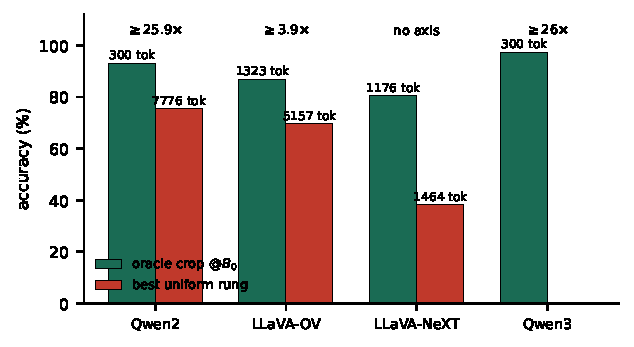
\includegraphics[width=\textwidth]{figs/fig_exchange.pdf}
\caption{\textbf{Allocation vs budget.} Oracle crop at the base budget (green) against the best
uniform rung each model reaches (red; token counts annotated). The exchange rate is the ratio of the
token counts at which the two arms score what they score; no uniform rung matches the crop, so each
rate is a lower bound.}
\label{fig:exchange}
\end{figure}

\begin{table}[h]\centering\footnotesize\setlength{\tabcolsep}{3pt}
\caption{\textbf{Allocation vs budget.} Placement effect = oracle crop $-$ random crop.}
\begin{tabular}{lccccc}
\toprule
model & oracle crop & random crop & placement effect & uniform ceiling & exchange rate\\
\midrule
Qwen2-VL-7B & 93.2\% @300 & 34.0\% & +59.2 & 75.4\% @7{,}776 & $\ge$25.9$\times$\\
LLaVA-OneVision-7B & 86.9\% @1{,}323 & 37.7\% & +49.2 & 69.6\% @5{,}157 & $\ge$3.9$\times$\\
LLaVA-NeXT-7B & 80.6\% @1{,}176 & 38.2\% & +42.4 & 38.2\% @1{,}464 & no axis\\
Qwen3-VL-2B & 97.4\% @300 & --- & +40.0 (attn$-$rand) & --- & $\ge$26$\times$\\
\bottomrule
\end{tabular}\label{tab:exchange}
\end{table}

\paragraph{What did not extend the crop.} Two attempts to buy the crop out of its cross-instance
limit failed, and both are charged in full. Adding the original image back costs $1.5\times$ the bar
once the localisation pass is counted and scores below the bar-matched crop alone on every stratum
(pooled $+4.2$ vs $+10.5$; cross $-10.5$ vs $-1.3$); the original dilutes the crop's attention more
than it restores the second object. Two full-resolution crops, funded by early-exit localisation and
boundary pruning at $101$--$104\%$ of the bar, help single further ($80.9$ vs $62.6$) but do not
clear on cross ($68.4$ vs $65.8$, $0$ of $2$ pre-registered).

\begin{table}[h]\centering\small
\caption{\textbf{Extensions of the crop, all charged in full.} Qwen3-VL-2B, \vstar, $n{=}191$; deltas
against the equal-compute bar. The funded 2-crop's pre-registered criterion did not pass ($0$ of
$2$).}
\begin{tabular}{lcccc}
\toprule
arm & cost vs bar & pooled & single & cross\\
\midrule
DWA crop (reference) & $1.0\times$ & \gd{$+10.5$} & \gd{$+18.3$} & $-1.3$\\
crop $+$ original & $1.5\times$ & $+4.2$ & $+13.9$ & \bad{$-10.5$}\\
2 crops $+$ original & $1.5\times$ & $+7.3$ & $+13.9$ & $-2.6$\\
4 crops $+$ original & $1.5\times$ & $+5.8$ & $+11.3$ & $-2.6$\\
funded 2-crop & $1.01$--$1.04\times$ & --- & \gd{$+18.3$} & $+2.6$\\
\bottomrule
\end{tabular}\label{tab:cropx}
\end{table}
; uses the macros defined there.

\section{Allocation beats budget}\label{app:allocation}

\paragraph{Protocol.} The \emph{exchange rate} compares an oracle crop at the base budget with the
best uniform rung each model can reach; a random crop of the same size bounds the placement effect
from below. No uniform rung reaches the crop arm on any model, so every rate is a lower bound set by
the model's token ceiling; LLaVA-NeXT has no resolution axis and is reported as such. The
native-resolution comparison runs the same items with the uniform arm free to spend the model's full
dynamic range, and the boundary test runs HR-Bench 4K, where targets are large enough to be
resolvable at the base budget.

\paragraph{Allocation vs budget.} The exchange rate is the ratio of the token counts at which the two
arms score what they score. An oracle crop at $300$ tokens reaches $97.4\%$ on Qwen3-VL-2B and
$93.2\%$ on Qwen2-VL-7B, while no uniform allocation on any rung up to $7{,}776$ tokens reaches the
crop arm (Qwen2's ceiling is $75.4\%$); the implied exchange rate is $\ge$26$\times$ and
$\ge$25.9$\times$ the same tokens spent uniformly, with the placement effect itself worth $+40.0$
and $+59.2$ points. At native resolution the same holds: a perfectly placed $600$-token crop beats
native dynamic resolution ($3{,}290$ tokens, $5.5\times$ the budget) by $+11.6$/$+16.2$ pooled. The
boundary is measured rather than assumed: allocation pays when the evidence is smaller than the
budget can resolve --- $71\%$ of \vstar\ targets are sub-token and oracle allocation is worth $+37.2$
points --- and costs when it is not, as on HR-Bench 4K, where allocation loses $8.8$ points because
discarded context dominates. The localizer is good in both regimes; what changes is whether acting
on it helps.

\begin{figure}[h]\centering
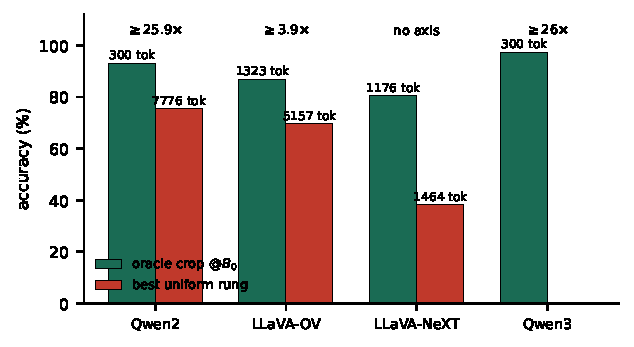
\includegraphics[width=\textwidth]{figs/fig_exchange.pdf}
\caption{\textbf{Allocation vs budget.} Oracle crop at the base budget (green) against the best
uniform rung each model reaches (red; token counts annotated). The exchange rate is the ratio of the
token counts at which the two arms score what they score; no uniform rung matches the crop, so each
rate is a lower bound.}
\label{fig:exchange}
\end{figure}

\begin{table}[h]\centering\footnotesize\setlength{\tabcolsep}{3pt}
\caption{\textbf{Allocation vs budget.} Placement effect = oracle crop $-$ random crop.}
\begin{tabular}{lccccc}
\toprule
model & oracle crop & random crop & placement effect & uniform ceiling & exchange rate\\
\midrule
Qwen2-VL-7B & 93.2\% @300 & 34.0\% & +59.2 & 75.4\% @7{,}776 & $\ge$25.9$\times$\\
LLaVA-OneVision-7B & 86.9\% @1{,}323 & 37.7\% & +49.2 & 69.6\% @5{,}157 & $\ge$3.9$\times$\\
LLaVA-NeXT-7B & 80.6\% @1{,}176 & 38.2\% & +42.4 & 38.2\% @1{,}464 & no axis\\
Qwen3-VL-2B & 97.4\% @300 & --- & +40.0 (attn$-$rand) & --- & $\ge$26$\times$\\
\bottomrule
\end{tabular}\label{tab:exchange}
\end{table}

\paragraph{What did not extend the crop.} Two attempts to buy the crop out of its cross-instance
limit failed, and both are charged in full. Adding the original image back costs $1.5\times$ the bar
once the localisation pass is counted and scores below the bar-matched crop alone on every stratum
(pooled $+4.2$ vs $+10.5$; cross $-10.5$ vs $-1.3$); the original dilutes the crop's attention more
than it restores the second object. Two full-resolution crops, funded by early-exit localisation and
boundary pruning at $101$--$104\%$ of the bar, help single further ($80.9$ vs $62.6$) but do not
clear on cross ($68.4$ vs $65.8$, $0$ of $2$ pre-registered).

\begin{table}[h]\centering\small
\caption{\textbf{Extensions of the crop, all charged in full.} Qwen3-VL-2B, \vstar, $n{=}191$; deltas
against the equal-compute bar. The funded 2-crop's pre-registered criterion did not pass ($0$ of
$2$).}
\begin{tabular}{lcccc}
\toprule
arm & cost vs bar & pooled & single & cross\\
\midrule
DWA crop (reference) & $1.0\times$ & \gd{$+10.5$} & \gd{$+18.3$} & $-1.3$\\
crop $+$ original & $1.5\times$ & $+4.2$ & $+13.9$ & \bad{$-10.5$}\\
2 crops $+$ original & $1.5\times$ & $+7.3$ & $+13.9$ & $-2.6$\\
4 crops $+$ original & $1.5\times$ & $+5.8$ & $+11.3$ & $-2.6$\\
funded 2-crop & $1.01$--$1.04\times$ & --- & \gd{$+18.3$} & $+2.6$\\
\bottomrule
\end{tabular}\label{tab:cropx}
\end{table}
; uses the macros defined there.

\section{Allocation beats budget}\label{app:allocation}

\paragraph{Protocol.} The \emph{exchange rate} compares an oracle crop at the base budget with the
best uniform rung each model can reach; a random crop of the same size bounds the placement effect
from below. No uniform rung reaches the crop arm on any model, so every rate is a lower bound set by
the model's token ceiling; LLaVA-NeXT has no resolution axis and is reported as such. The
native-resolution comparison runs the same items with the uniform arm free to spend the model's full
dynamic range, and the boundary test runs HR-Bench 4K, where targets are large enough to be
resolvable at the base budget.

\paragraph{Allocation vs budget.} The exchange rate is the ratio of the token counts at which the two
arms score what they score. An oracle crop at $300$ tokens reaches $97.4\%$ on Qwen3-VL-2B and
$93.2\%$ on Qwen2-VL-7B, while no uniform allocation on any rung up to $7{,}776$ tokens reaches the
crop arm (Qwen2's ceiling is $75.4\%$); the implied exchange rate is $\ge$26$\times$ and
$\ge$25.9$\times$ the same tokens spent uniformly, with the placement effect itself worth $+40.0$
and $+59.2$ points. At native resolution the same holds: a perfectly placed $600$-token crop beats
native dynamic resolution ($3{,}290$ tokens, $5.5\times$ the budget) by $+11.6$/$+16.2$ pooled. The
boundary is measured rather than assumed: allocation pays when the evidence is smaller than the
budget can resolve --- $71\%$ of \vstar\ targets are sub-token and oracle allocation is worth $+37.2$
points --- and costs when it is not, as on HR-Bench 4K, where allocation loses $8.8$ points because
discarded context dominates. The localizer is good in both regimes; what changes is whether acting
on it helps.

\begin{figure}[h]\centering
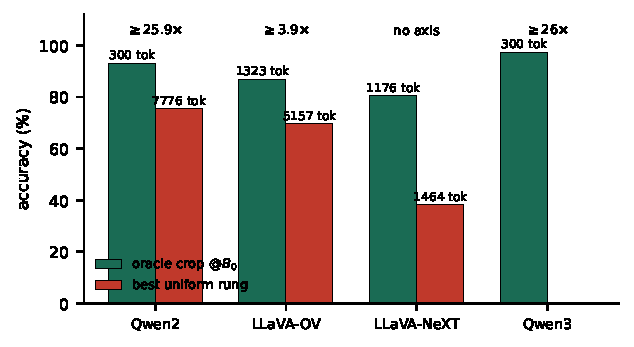
\includegraphics[width=\textwidth]{figs/fig_exchange.pdf}
\caption{\textbf{Allocation vs budget.} Oracle crop at the base budget (green) against the best
uniform rung each model reaches (red; token counts annotated). The exchange rate is the ratio of the
token counts at which the two arms score what they score; no uniform rung matches the crop, so each
rate is a lower bound.}
\label{fig:exchange}
\end{figure}

\begin{table}[h]\centering\footnotesize\setlength{\tabcolsep}{3pt}
\caption{\textbf{Allocation vs budget.} Placement effect = oracle crop $-$ random crop.}
\begin{tabular}{lccccc}
\toprule
model & oracle crop & random crop & placement effect & uniform ceiling & exchange rate\\
\midrule
Qwen2-VL-7B & 93.2\% @300 & 34.0\% & +59.2 & 75.4\% @7{,}776 & $\ge$25.9$\times$\\
LLaVA-OneVision-7B & 86.9\% @1{,}323 & 37.7\% & +49.2 & 69.6\% @5{,}157 & $\ge$3.9$\times$\\
LLaVA-NeXT-7B & 80.6\% @1{,}176 & 38.2\% & +42.4 & 38.2\% @1{,}464 & no axis\\
Qwen3-VL-2B & 97.4\% @300 & --- & +40.0 (attn$-$rand) & --- & $\ge$26$\times$\\
\bottomrule
\end{tabular}\label{tab:exchange}
\end{table}

\paragraph{What did not extend the crop.} Two attempts to buy the crop out of its cross-instance
limit failed, and both are charged in full. Adding the original image back costs $1.5\times$ the bar
once the localisation pass is counted and scores below the bar-matched crop alone on every stratum
(pooled $+4.2$ vs $+10.5$; cross $-10.5$ vs $-1.3$); the original dilutes the crop's attention more
than it restores the second object. Two full-resolution crops, funded by early-exit localisation and
boundary pruning at $101$--$104\%$ of the bar, help single further ($80.9$ vs $62.6$) but do not
clear on cross ($68.4$ vs $65.8$, $0$ of $2$ pre-registered).

\begin{table}[h]\centering\small
\caption{\textbf{Extensions of the crop, all charged in full.} Qwen3-VL-2B, \vstar, $n{=}191$; deltas
against the equal-compute bar. The funded 2-crop's pre-registered criterion did not pass ($0$ of
$2$).}
\begin{tabular}{lcccc}
\toprule
arm & cost vs bar & pooled & single & cross\\
\midrule
DWA crop (reference) & $1.0\times$ & \gd{$+10.5$} & \gd{$+18.3$} & $-1.3$\\
crop $+$ original & $1.5\times$ & $+4.2$ & $+13.9$ & \bad{$-10.5$}\\
2 crops $+$ original & $1.5\times$ & $+7.3$ & $+13.9$ & $-2.6$\\
4 crops $+$ original & $1.5\times$ & $+5.8$ & $+11.3$ & $-2.6$\\
funded 2-crop & $1.01$--$1.04\times$ & --- & \gd{$+18.3$} & $+2.6$\\
\bottomrule
\end{tabular}\label{tab:cropx}
\end{table}
; uses the macros defined there.

\section{Allocation beats budget}\label{app:allocation}

\paragraph{Protocol.} The \emph{exchange rate} compares an oracle crop at the base budget with the
best uniform rung each model can reach; a random crop of the same size bounds the placement effect
from below. No uniform rung reaches the crop arm on any model, so every rate is a lower bound set by
the model's token ceiling; LLaVA-NeXT has no resolution axis and is reported as such. The
native-resolution comparison runs the same items with the uniform arm free to spend the model's full
dynamic range, and the boundary test runs HR-Bench 4K, where targets are large enough to be
resolvable at the base budget.

\paragraph{Allocation vs budget.} The exchange rate is the ratio of the token counts at which the two
arms score what they score. An oracle crop at $300$ tokens reaches $97.4\%$ on Qwen3-VL-2B and
$93.2\%$ on Qwen2-VL-7B, while no uniform allocation on any rung up to $7{,}776$ tokens reaches the
crop arm (Qwen2's ceiling is $75.4\%$); the implied exchange rate is $\ge$26$\times$ and
$\ge$25.9$\times$ the same tokens spent uniformly, with the placement effect itself worth $+40.0$
and $+59.2$ points. At native resolution the same holds: a perfectly placed $600$-token crop beats
native dynamic resolution ($3{,}290$ tokens, $5.5\times$ the budget) by $+11.6$/$+16.2$ pooled. The
boundary is measured rather than assumed: allocation pays when the evidence is smaller than the
budget can resolve --- $71\%$ of \vstar\ targets are sub-token and oracle allocation is worth $+37.2$
points --- and costs when it is not, as on HR-Bench 4K, where allocation loses $8.8$ points because
discarded context dominates. The localizer is good in both regimes; what changes is whether acting
on it helps.

\begin{figure}[h]\centering
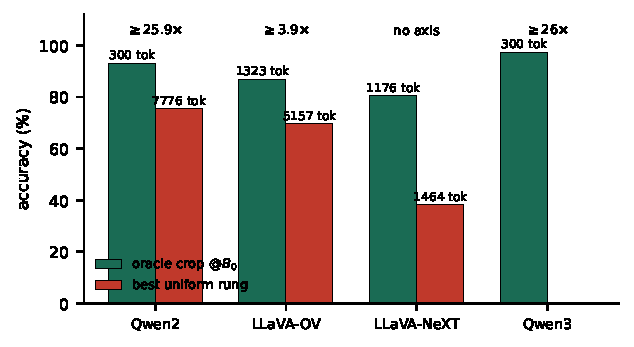
\includegraphics[width=\textwidth]{figs/fig_exchange.pdf}
\caption{\textbf{Allocation vs budget.} Oracle crop at the base budget (green) against the best
uniform rung each model reaches (red; token counts annotated). The exchange rate is the ratio of the
token counts at which the two arms score what they score; no uniform rung matches the crop, so each
rate is a lower bound.}
\label{fig:exchange}
\end{figure}

\begin{table}[h]\centering\footnotesize\setlength{\tabcolsep}{3pt}
\caption{\textbf{Allocation vs budget.} Placement effect = oracle crop $-$ random crop.}
\begin{tabular}{lccccc}
\toprule
model & oracle crop & random crop & placement effect & uniform ceiling & exchange rate\\
\midrule
Qwen2-VL-7B & 93.2\% @300 & 34.0\% & +59.2 & 75.4\% @7{,}776 & $\ge$25.9$\times$\\
LLaVA-OneVision-7B & 86.9\% @1{,}323 & 37.7\% & +49.2 & 69.6\% @5{,}157 & $\ge$3.9$\times$\\
LLaVA-NeXT-7B & 80.6\% @1{,}176 & 38.2\% & +42.4 & 38.2\% @1{,}464 & no axis\\
Qwen3-VL-2B & 97.4\% @300 & --- & +40.0 (attn$-$rand) & --- & $\ge$26$\times$\\
\bottomrule
\end{tabular}\label{tab:exchange}
\end{table}

\paragraph{What did not extend the crop.} Two attempts to buy the crop out of its cross-instance
limit failed, and both are charged in full. Adding the original image back costs $1.5\times$ the bar
once the localisation pass is counted and scores below the bar-matched crop alone on every stratum
(pooled $+4.2$ vs $+10.5$; cross $-10.5$ vs $-1.3$); the original dilutes the crop's attention more
than it restores the second object. Two full-resolution crops, funded by early-exit localisation and
boundary pruning at $101$--$104\%$ of the bar, help single further ($80.9$ vs $62.6$) but do not
clear on cross ($68.4$ vs $65.8$, $0$ of $2$ pre-registered).

\begin{table}[h]\centering\small
\caption{\textbf{Extensions of the crop, all charged in full.} Qwen3-VL-2B, \vstar, $n{=}191$; deltas
against the equal-compute bar. The funded 2-crop's pre-registered criterion did not pass ($0$ of
$2$).}
\begin{tabular}{lcccc}
\toprule
arm & cost vs bar & pooled & single & cross\\
\midrule
DWA crop (reference) & $1.0\times$ & \gd{$+10.5$} & \gd{$+18.3$} & $-1.3$\\
crop $+$ original & $1.5\times$ & $+4.2$ & $+13.9$ & \bad{$-10.5$}\\
2 crops $+$ original & $1.5\times$ & $+7.3$ & $+13.9$ & $-2.6$\\
4 crops $+$ original & $1.5\times$ & $+5.8$ & $+11.3$ & $-2.6$\\
funded 2-crop & $1.01$--$1.04\times$ & --- & \gd{$+18.3$} & $+2.6$\\
\bottomrule
\end{tabular}\label{tab:cropx}
\end{table}
